% Options for packages loaded elsewhere
\PassOptionsToPackage{unicode}{hyperref}
\PassOptionsToPackage{hyphens}{url}
%
\documentclass[
]{article}
\usepackage{amsmath,amssymb}
\usepackage{iftex}
\ifPDFTeX
  \usepackage[T1]{fontenc}
  \usepackage[utf8]{inputenc}
  \usepackage{textcomp} % provide euro and other symbols
\else % if luatex or xetex
  \usepackage{unicode-math} % this also loads fontspec
  \defaultfontfeatures{Scale=MatchLowercase}
  \defaultfontfeatures[\rmfamily]{Ligatures=TeX,Scale=1}
\fi
\usepackage{lmodern}
\ifPDFTeX\else
  % xetex/luatex font selection
\fi
% Use upquote if available, for straight quotes in verbatim environments
\IfFileExists{upquote.sty}{\usepackage{upquote}}{}
\IfFileExists{microtype.sty}{% use microtype if available
  \usepackage[]{microtype}
  \UseMicrotypeSet[protrusion]{basicmath} % disable protrusion for tt fonts
}{}
\makeatletter
\@ifundefined{KOMAClassName}{% if non-KOMA class
  \IfFileExists{parskip.sty}{%
    \usepackage{parskip}
  }{% else
    \setlength{\parindent}{0pt}
    \setlength{\parskip}{6pt plus 2pt minus 1pt}}
}{% if KOMA class
  \KOMAoptions{parskip=half}}
\makeatother
\usepackage{xcolor}
\usepackage[margin=1in]{geometry}
\usepackage{color}
\usepackage{fancyvrb}
\newcommand{\VerbBar}{|}
\newcommand{\VERB}{\Verb[commandchars=\\\{\}]}
\DefineVerbatimEnvironment{Highlighting}{Verbatim}{commandchars=\\\{\}}
% Add ',fontsize=\small' for more characters per line
\usepackage{framed}
\definecolor{shadecolor}{RGB}{248,248,248}
\newenvironment{Shaded}{\begin{snugshade}}{\end{snugshade}}
\newcommand{\AlertTok}[1]{\textcolor[rgb]{0.94,0.16,0.16}{#1}}
\newcommand{\AnnotationTok}[1]{\textcolor[rgb]{0.56,0.35,0.01}{\textbf{\textit{#1}}}}
\newcommand{\AttributeTok}[1]{\textcolor[rgb]{0.13,0.29,0.53}{#1}}
\newcommand{\BaseNTok}[1]{\textcolor[rgb]{0.00,0.00,0.81}{#1}}
\newcommand{\BuiltInTok}[1]{#1}
\newcommand{\CharTok}[1]{\textcolor[rgb]{0.31,0.60,0.02}{#1}}
\newcommand{\CommentTok}[1]{\textcolor[rgb]{0.56,0.35,0.01}{\textit{#1}}}
\newcommand{\CommentVarTok}[1]{\textcolor[rgb]{0.56,0.35,0.01}{\textbf{\textit{#1}}}}
\newcommand{\ConstantTok}[1]{\textcolor[rgb]{0.56,0.35,0.01}{#1}}
\newcommand{\ControlFlowTok}[1]{\textcolor[rgb]{0.13,0.29,0.53}{\textbf{#1}}}
\newcommand{\DataTypeTok}[1]{\textcolor[rgb]{0.13,0.29,0.53}{#1}}
\newcommand{\DecValTok}[1]{\textcolor[rgb]{0.00,0.00,0.81}{#1}}
\newcommand{\DocumentationTok}[1]{\textcolor[rgb]{0.56,0.35,0.01}{\textbf{\textit{#1}}}}
\newcommand{\ErrorTok}[1]{\textcolor[rgb]{0.64,0.00,0.00}{\textbf{#1}}}
\newcommand{\ExtensionTok}[1]{#1}
\newcommand{\FloatTok}[1]{\textcolor[rgb]{0.00,0.00,0.81}{#1}}
\newcommand{\FunctionTok}[1]{\textcolor[rgb]{0.13,0.29,0.53}{\textbf{#1}}}
\newcommand{\ImportTok}[1]{#1}
\newcommand{\InformationTok}[1]{\textcolor[rgb]{0.56,0.35,0.01}{\textbf{\textit{#1}}}}
\newcommand{\KeywordTok}[1]{\textcolor[rgb]{0.13,0.29,0.53}{\textbf{#1}}}
\newcommand{\NormalTok}[1]{#1}
\newcommand{\OperatorTok}[1]{\textcolor[rgb]{0.81,0.36,0.00}{\textbf{#1}}}
\newcommand{\OtherTok}[1]{\textcolor[rgb]{0.56,0.35,0.01}{#1}}
\newcommand{\PreprocessorTok}[1]{\textcolor[rgb]{0.56,0.35,0.01}{\textit{#1}}}
\newcommand{\RegionMarkerTok}[1]{#1}
\newcommand{\SpecialCharTok}[1]{\textcolor[rgb]{0.81,0.36,0.00}{\textbf{#1}}}
\newcommand{\SpecialStringTok}[1]{\textcolor[rgb]{0.31,0.60,0.02}{#1}}
\newcommand{\StringTok}[1]{\textcolor[rgb]{0.31,0.60,0.02}{#1}}
\newcommand{\VariableTok}[1]{\textcolor[rgb]{0.00,0.00,0.00}{#1}}
\newcommand{\VerbatimStringTok}[1]{\textcolor[rgb]{0.31,0.60,0.02}{#1}}
\newcommand{\WarningTok}[1]{\textcolor[rgb]{0.56,0.35,0.01}{\textbf{\textit{#1}}}}
\usepackage{graphicx}
\makeatletter
\def\maxwidth{\ifdim\Gin@nat@width>\linewidth\linewidth\else\Gin@nat@width\fi}
\def\maxheight{\ifdim\Gin@nat@height>\textheight\textheight\else\Gin@nat@height\fi}
\makeatother
% Scale images if necessary, so that they will not overflow the page
% margins by default, and it is still possible to overwrite the defaults
% using explicit options in \includegraphics[width, height, ...]{}
\setkeys{Gin}{width=\maxwidth,height=\maxheight,keepaspectratio}
% Set default figure placement to htbp
\makeatletter
\def\fps@figure{htbp}
\makeatother
\setlength{\emergencystretch}{3em} % prevent overfull lines
\providecommand{\tightlist}{%
  \setlength{\itemsep}{0pt}\setlength{\parskip}{0pt}}
\setcounter{secnumdepth}{5}
\usepackage{booktabs}
\usepackage{longtable}
\usepackage{array}
\usepackage{multirow}
\usepackage{wrapfig}
\usepackage{float}
\usepackage{colortbl}
\usepackage{pdflscape}
\usepackage{tabu}
\usepackage{threeparttable}
\usepackage{threeparttablex}
\usepackage[normalem]{ulem}
\usepackage{makecell}
\usepackage{xcolor}
\ifLuaTeX
  \usepackage{selnolig}  % disable illegal ligatures
\fi
\usepackage[]{natbib}
\bibliographystyle{plainnat}
\usepackage{bookmark}
\IfFileExists{xurl.sty}{\usepackage{xurl}}{} % add URL line breaks if available
\urlstyle{same}
\hypersetup{
  pdftitle={Causal Inference with Continuous Exposures: A Tutorial with Application to ICU Data: Simulation},
  pdfauthor={M Ehsan Karim},
  hidelinks,
  pdfcreator={LaTeX via pandoc}}

\title{Causal Inference with Continuous Exposures: A Tutorial with
Application to ICU Data: Simulation}
\author{M Ehsan Karim}
\date{}

\begin{document}
\maketitle

\section{Simulate Data for Analysis}\label{simulate-data-for-analysis}

We begin by simulating data with known causal relationships. This allows
us to assess how well our methods estimate the true effects. We use the
\texttt{simcausal} package, which defines data generation based on a
Directed Acyclic Graph (DAG). We simulate a dataset where:

\begin{itemize}
\tightlist
\item
  \texttt{A} is the continuous exposure, generated as a function of
  confounders \texttt{C1}, \texttt{C2}
\item
  \texttt{Y} is the binary outcome, generated as a function of
  \texttt{A}, \texttt{C1}, and \texttt{C2}
\item
  \texttt{C1}, \texttt{C2} are measured confounders
\end{itemize}

The true conditional effect of A on Y (log-odds ratio) is set to \(0.4\)
in the simulation.

\begin{Shaded}
\begin{Highlighting}[]
\FunctionTok{library}\NormalTok{(simcausal)}
\FunctionTok{set.seed}\NormalTok{(}\DecValTok{123}\NormalTok{)}
\NormalTok{D }\OtherTok{\textless{}{-}} \FunctionTok{DAG.empty}\NormalTok{() }\SpecialCharTok{+}
  \FunctionTok{node}\NormalTok{(}\StringTok{"C1"}\NormalTok{, }\AttributeTok{distr =} \StringTok{"rnorm"}\NormalTok{, }\AttributeTok{mean =} \DecValTok{0}\NormalTok{, }\AttributeTok{sd =} \DecValTok{1}\NormalTok{) }\SpecialCharTok{+}
  \FunctionTok{node}\NormalTok{(}\StringTok{"C2"}\NormalTok{, }\AttributeTok{distr =} \StringTok{"rbern"}\NormalTok{, }\AttributeTok{prob =} \FloatTok{0.5}\NormalTok{) }\SpecialCharTok{+}
  \FunctionTok{node}\NormalTok{(}\StringTok{"A"}\NormalTok{, }\AttributeTok{distr =} \StringTok{"rnorm"}\NormalTok{, }\AttributeTok{mean =} \FloatTok{0.5} \SpecialCharTok{*}\NormalTok{ C1 }\SpecialCharTok{+} \FloatTok{0.3} \SpecialCharTok{*}\NormalTok{ C2, }\AttributeTok{sd =} \FunctionTok{exp}\NormalTok{(.}\DecValTok{8}\SpecialCharTok{*}\NormalTok{C1)) }\SpecialCharTok{+}  
  \CommentTok{\# Exposure depends on confounders (Heteroscedastic)}
  \CommentTok{\# alternative could be to simulate from a gamma distribution:}
  \CommentTok{\# node("A", distr = "rgamma", shape = 2 + C1, scale = 1) +}
  \FunctionTok{node}\NormalTok{(}\StringTok{"Y"}\NormalTok{, }\AttributeTok{distr =} \StringTok{"rbern"}\NormalTok{, }\AttributeTok{prob =} \FunctionTok{plogis}\NormalTok{(}\FloatTok{0.4} \SpecialCharTok{*}\NormalTok{ A }\SpecialCharTok{+} \FloatTok{0.5} \SpecialCharTok{*}\NormalTok{ C1 }\SpecialCharTok{{-}} \FloatTok{0.3} \SpecialCharTok{*}\NormalTok{ C2))  }
  \CommentTok{\# Known true effect of A on Y}
\NormalTok{Dset }\OtherTok{\textless{}{-}} \FunctionTok{set.DAG}\NormalTok{(D, }\AttributeTok{n.test =} \FloatTok{1e6}\NormalTok{)}

\CommentTok{\# Plot DAG}
\FunctionTok{plotDAG}\NormalTok{(Dset)}
\end{Highlighting}
\end{Shaded}

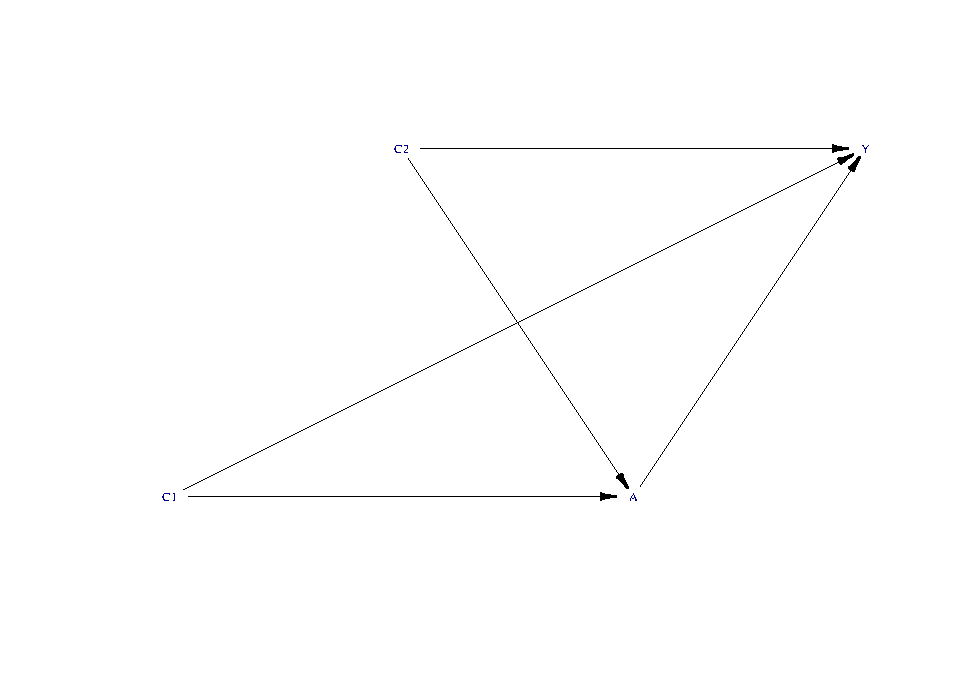
\includegraphics{simulation_files/figure-latex/simulate-data-1.pdf}

\begin{Shaded}
\begin{Highlighting}[]
\CommentTok{\# Simulate data}
\NormalTok{simdata }\OtherTok{\textless{}{-}} \FunctionTok{sim}\NormalTok{(Dset, }\AttributeTok{n =} \DecValTok{1000}\NormalTok{)}
\end{Highlighting}
\end{Shaded}

Let's visualize the distribution of our continuous exposure A.

\begin{Shaded}
\begin{Highlighting}[]
\FunctionTok{library}\NormalTok{(ggplot2)}

\CommentTok{\# Histogram with density overlay}
\FunctionTok{ggplot}\NormalTok{(simdata, }\FunctionTok{aes}\NormalTok{(}\AttributeTok{x =}\NormalTok{ A)) }\SpecialCharTok{+}
  \FunctionTok{geom\_histogram}\NormalTok{(}\FunctionTok{aes}\NormalTok{(}\AttributeTok{y =}\NormalTok{ ..density..), }\AttributeTok{bins =} \DecValTok{40}\NormalTok{, }\AttributeTok{fill =} \StringTok{"steelblue"}\NormalTok{, }\AttributeTok{alpha =} \FloatTok{0.6}\NormalTok{) }\SpecialCharTok{+}
  \FunctionTok{geom\_density}\NormalTok{(}\AttributeTok{color =} \StringTok{"black"}\NormalTok{, }\AttributeTok{linewidth =} \DecValTok{1}\NormalTok{) }\SpecialCharTok{+}
  \FunctionTok{labs}\NormalTok{(}\AttributeTok{title =} \StringTok{"Distribution of Exposure A"}\NormalTok{, }\AttributeTok{x =} \StringTok{"A"}\NormalTok{, }\AttributeTok{y =} \StringTok{"Density"}\NormalTok{) }\SpecialCharTok{+}
  \FunctionTok{theme\_minimal}\NormalTok{()}
\end{Highlighting}
\end{Shaded}

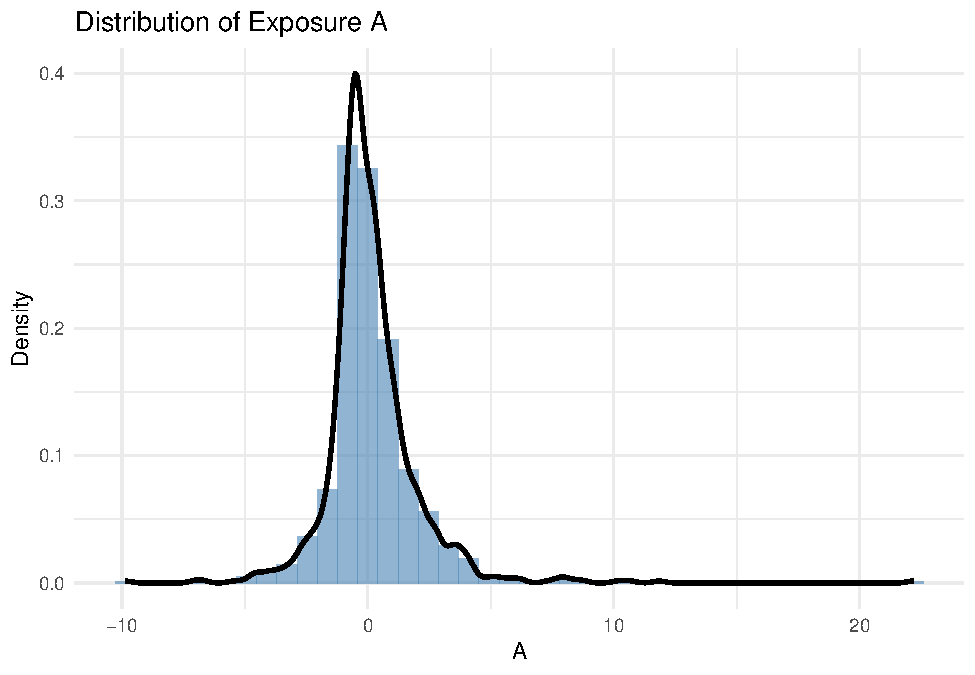
\includegraphics{simulation_files/figure-latex/plot-1.pdf}

\subsection{Method 1: Normal Model for
Exposure}\label{method-1-normal-model-for-exposure}

This method assumes that the exposure is normally distributed with
constant variance (homoscedastic).

\begin{itemize}
\tightlist
\item
  Fit a marginal model for numerator (A \textasciitilde{} 1)
\item
  Fit a conditional model for denominator (A \textasciitilde{} C1 + C2)
\item
  Use normal density to compute stabilized weights
\end{itemize}

\begin{Shaded}
\begin{Highlighting}[]
\CommentTok{\# Marginal model}
\NormalTok{marg\_model }\OtherTok{\textless{}{-}} \FunctionTok{lm}\NormalTok{(A }\SpecialCharTok{\textasciitilde{}} \DecValTok{1}\NormalTok{, }\AttributeTok{data =}\NormalTok{ simdata)}
\NormalTok{mu\_num }\OtherTok{\textless{}{-}} \FunctionTok{predict}\NormalTok{(marg\_model)}
\NormalTok{sd\_num }\OtherTok{\textless{}{-}} \FunctionTok{sd}\NormalTok{(}\FunctionTok{residuals}\NormalTok{(marg\_model))}

\CommentTok{\# Conditional model}
\NormalTok{cond\_model }\OtherTok{\textless{}{-}} \FunctionTok{lm}\NormalTok{(A }\SpecialCharTok{\textasciitilde{}}\NormalTok{ C1 }\SpecialCharTok{+}\NormalTok{ C2, }\AttributeTok{data =}\NormalTok{ simdata)}
\NormalTok{mu\_denom }\OtherTok{\textless{}{-}} \FunctionTok{predict}\NormalTok{(cond\_model)}
\NormalTok{sd\_denom }\OtherTok{\textless{}{-}} \FunctionTok{sd}\NormalTok{(}\FunctionTok{residuals}\NormalTok{(cond\_model))}

\CommentTok{\# Compute densities}
\NormalTok{f\_num }\OtherTok{\textless{}{-}} \FunctionTok{dnorm}\NormalTok{(simdata}\SpecialCharTok{$}\NormalTok{A, }\AttributeTok{mean =}\NormalTok{ mu\_num, }\AttributeTok{sd =}\NormalTok{ sd\_num)}
\NormalTok{f\_denom }\OtherTok{\textless{}{-}} \FunctionTok{dnorm}\NormalTok{(simdata}\SpecialCharTok{$}\NormalTok{A, }\AttributeTok{mean =}\NormalTok{ mu\_denom, }\AttributeTok{sd =}\NormalTok{ sd\_denom)}

\CommentTok{\# Compute stabilized weights}
\NormalTok{simdata}\SpecialCharTok{$}\NormalTok{sw\_normal }\OtherTok{\textless{}{-}}\NormalTok{ f\_num }\SpecialCharTok{/}\NormalTok{ f\_denom}
\end{Highlighting}
\end{Shaded}

\subsection{Method 2: Quantile Binning
Approach}\label{method-2-quantile-binning-approach}

This approach does not assume a distributional form and is robust to
outliers and heteroscedasticity.

\begin{itemize}
\tightlist
\item
  Discretize the exposure into quantiles
\item
  Estimate conditional probability of each quantile using a multinomial
  logistic model
\item
  Use inverse of predicted conditional probabilities to compute weights
\end{itemize}

\begin{Shaded}
\begin{Highlighting}[]
\CommentTok{\# Categorize A into 10 quantiles}
\NormalTok{simdata}\SpecialCharTok{$}\NormalTok{qbin }\OtherTok{\textless{}{-}} \FunctionTok{cut}\NormalTok{(simdata}\SpecialCharTok{$}\NormalTok{A, }
                    \AttributeTok{breaks =} \FunctionTok{quantile}\NormalTok{(simdata}\SpecialCharTok{$}\NormalTok{A, }
                                      \AttributeTok{probs =} \FunctionTok{seq}\NormalTok{(}\DecValTok{0}\NormalTok{, }\DecValTok{1}\NormalTok{, }\FloatTok{0.1}\NormalTok{)), }
                    \AttributeTok{include.lowest =} \ConstantTok{TRUE}\NormalTok{, }\AttributeTok{labels =} \ConstantTok{FALSE}\NormalTok{)}

\CommentTok{\# Fit multinomial logistic regression for P(qbin | C)}
\FunctionTok{library}\NormalTok{(nnet)}
\NormalTok{denom\_model }\OtherTok{\textless{}{-}} \FunctionTok{multinom}\NormalTok{(}\FunctionTok{factor}\NormalTok{(qbin) }\SpecialCharTok{\textasciitilde{}}\NormalTok{ C1 }\SpecialCharTok{+}\NormalTok{ C2, }
                        \AttributeTok{data =}\NormalTok{ simdata, }\AttributeTok{trace =} \ConstantTok{FALSE}\NormalTok{)}
\NormalTok{p\_denom }\OtherTok{\textless{}{-}} \FunctionTok{predict}\NormalTok{(denom\_model, }\AttributeTok{type =} \StringTok{"probs"}\NormalTok{)}
\NormalTok{row\_idx }\OtherTok{\textless{}{-}} \FunctionTok{cbind}\NormalTok{(}\DecValTok{1}\SpecialCharTok{:}\FunctionTok{nrow}\NormalTok{(simdata), simdata}\SpecialCharTok{$}\NormalTok{qbin)}
\NormalTok{p\_denom\_val }\OtherTok{\textless{}{-}}\NormalTok{ p\_denom[row\_idx]}

\CommentTok{\# Numerator is uniform across quantiles}
\NormalTok{p\_num\_val }\OtherTok{\textless{}{-}} \DecValTok{1} \SpecialCharTok{/} \DecValTok{10}

\CommentTok{\# Stabilized weights}
\NormalTok{simdata}\SpecialCharTok{$}\NormalTok{sw\_qbin }\OtherTok{\textless{}{-}}\NormalTok{ p\_num\_val }\SpecialCharTok{/}\NormalTok{ p\_denom\_val}
\end{Highlighting}
\end{Shaded}

\subsection{Weighted Outcome Model}\label{weighted-outcome-model}

With IPW weights, we estimate the marginal effect of A on Y using a
weighted logistic regression model:
\(logit(P(Y=1)) = \beta_0 + \beta_A A\). The weights create a
pseudo-population where confounding between A and (\(C_1\), \(C_2\)) is
removed. The coefficient \(\beta_A\) is our estimate of the marginal
log-odds ratio.

\begin{Shaded}
\begin{Highlighting}[]
\CommentTok{\# Weighted outcome model using logistic regression}
\NormalTok{model\_normal }\OtherTok{\textless{}{-}} \FunctionTok{glm}\NormalTok{(Y }\SpecialCharTok{\textasciitilde{}}\NormalTok{ A, }
                    \AttributeTok{family =} \FunctionTok{binomial}\NormalTok{(), }
                    \AttributeTok{data =}\NormalTok{ simdata, }
                    \AttributeTok{weights =}\NormalTok{ sw\_normal)}
\NormalTok{model\_qbin }\OtherTok{\textless{}{-}} \FunctionTok{glm}\NormalTok{(Y }\SpecialCharTok{\textasciitilde{}}\NormalTok{ A, }
                  \AttributeTok{family =} \FunctionTok{binomial}\NormalTok{(), }
                  \AttributeTok{data =}\NormalTok{ simdata, }
                  \AttributeTok{weights =}\NormalTok{ sw\_qbin)}

\CommentTok{\# Summary of models}
\FunctionTok{require}\NormalTok{(Publish)}
\FunctionTok{publish}\NormalTok{(model\_normal)}
\end{Highlighting}
\end{Shaded}

\begin{verbatim}
##  Variable Units OddsRatio       CI.95 p-value 
##         A            1.43 [1.36;1.51] < 1e-04
\end{verbatim}

\begin{Shaded}
\begin{Highlighting}[]
\FunctionTok{publish}\NormalTok{(model\_qbin)}
\end{Highlighting}
\end{Shaded}

\begin{verbatim}
##  Variable Units OddsRatio       CI.95 p-value 
##         A            1.92 [1.71;2.17] < 1e-04
\end{verbatim}

\subsection{Method 3: TMLE}\label{method-3-tmle}

TMLE is a doubly robust, semi-parametric method. Doubly robust means it
provides unbiased estimates if either the outcome model \(E[Y|A,W]\) or
the exposure mechanism model \(P(A|W)\) is correctly specified. We use
the \texttt{tmle3} package suite. TMLE involves:

\begin{enumerate}
\def\labelenumi{\arabic{enumi}.}
\tightlist
\item
  Initial estimation of the outcome mechanism (\(Q(A,W)\)) and exposure
  mechanism (\(g(A|W)\)).
\item
  A ``targeting'' step that updates \(Q(A,W)\) to optimize the
  bias-variance tradeoff for the parameter of interest.
\end{enumerate}

We'll estimate the effect of a small shift, \(\delta=0.1\), in exposure
A. The parameter of interest from tmle\_shift with a binary outcome is
often related to a coefficient in a marginal structural model like
\(logit P(Y(a)) = \alpha_0 + \alpha_1 a\). The raw TMLE estimate (psi)
will be for the effect of this \(\delta\) shift (i.e.,
\(\alpha_1 \times \delta\)). To get \(\alpha_1\) (the log-odds ratio per
1-unit increase in A), we divide psi by \(\delta\).

\begin{Shaded}
\begin{Highlighting}[]
\NormalTok{\{}
  \FunctionTok{library}\NormalTok{(tmle3)}
  \FunctionTok{library}\NormalTok{(tmle3shift)}
  \FunctionTok{library}\NormalTok{(sl3)}
  \FunctionTok{library}\NormalTok{(data.table)}

  \CommentTok{\# Define nodes}
\NormalTok{  node\_list }\OtherTok{\textless{}{-}} \FunctionTok{list}\NormalTok{(}
    \AttributeTok{W =} \FunctionTok{c}\NormalTok{(}\StringTok{"C1"}\NormalTok{, }\StringTok{"C2"}\NormalTok{),}
    \AttributeTok{A =} \StringTok{"A"}\NormalTok{,}
    \AttributeTok{Y =} \StringTok{"Y"}
\NormalTok{  )}

  \CommentTok{\# Define trained learners (scoped inside this block)}
\NormalTok{  glm\_learner }\OtherTok{\textless{}{-}} \FunctionTok{make\_learner}\NormalTok{(Lrnr\_glm)}
\NormalTok{  learner\_list }\OtherTok{\textless{}{-}} \FunctionTok{list}\NormalTok{(}
    \AttributeTok{Y =}\NormalTok{ glm\_learner,}
    \AttributeTok{A =}\NormalTok{ glm\_learner}
\NormalTok{  )}

  \CommentTok{\# Shift function using tmle\_task}
\NormalTok{  tmle\_spec }\OtherTok{\textless{}{-}} \FunctionTok{tmle\_shift}\NormalTok{(}
    \AttributeTok{delta =} \FloatTok{0.1}\NormalTok{,}
    \AttributeTok{shift\_fxn =} \ControlFlowTok{function}\NormalTok{(tmle\_task, delta, ...) \{}
\NormalTok{      a }\OtherTok{\textless{}{-}}\NormalTok{ tmle\_task}\SpecialCharTok{$}\FunctionTok{get\_tmle\_node}\NormalTok{(}\StringTok{"A"}\NormalTok{)}
\NormalTok{      a }\SpecialCharTok{+}\NormalTok{ delta}
\NormalTok{    \},}
    \AttributeTok{max\_shift =} \DecValTok{1}
\NormalTok{  )}
  
\NormalTok{  future}\SpecialCharTok{::}\FunctionTok{plan}\NormalTok{(future}\SpecialCharTok{::}\NormalTok{sequential)}

  \CommentTok{\# Run TMLE}
\NormalTok{  tmle\_fit }\OtherTok{\textless{}{-}} \FunctionTok{tmle3}\NormalTok{(}
\NormalTok{    tmle\_spec,}
    \AttributeTok{data =} \FunctionTok{as.data.table}\NormalTok{(simdata),}
    \AttributeTok{node\_list =}\NormalTok{ node\_list,}
    \AttributeTok{learner\_list =}\NormalTok{ learner\_list}
\NormalTok{  )}

  \CommentTok{\# Print estimate}
  \FunctionTok{print}\NormalTok{(}\FunctionTok{exp}\NormalTok{(tmle\_fit}\SpecialCharTok{$}\NormalTok{estimates[[}\DecValTok{1}\NormalTok{]]}\SpecialCharTok{$}\NormalTok{psi))}
\NormalTok{\}}
\end{Highlighting}
\end{Shaded}

\begin{verbatim}
## [1] 1.761697
\end{verbatim}

\begin{Shaded}
\begin{Highlighting}[]
\CommentTok{\# Extract psi and IC}
\NormalTok{psi }\OtherTok{\textless{}{-}}\NormalTok{ tmle\_fit}\SpecialCharTok{$}\NormalTok{estimates[[}\DecValTok{1}\NormalTok{]]}\SpecialCharTok{$}\NormalTok{psi}
\NormalTok{IC }\OtherTok{\textless{}{-}}\NormalTok{ tmle\_fit}\SpecialCharTok{$}\NormalTok{estimates[[}\DecValTok{1}\NormalTok{]]}\SpecialCharTok{$}\NormalTok{IC}

\CommentTok{\# Compute standard error}
\NormalTok{se }\OtherTok{\textless{}{-}} \FunctionTok{sd}\NormalTok{(IC) }\SpecialCharTok{/} \FunctionTok{sqrt}\NormalTok{(}\FunctionTok{length}\NormalTok{(IC))}

\CommentTok{\# 95\% confidence interval}
\NormalTok{ci }\OtherTok{\textless{}{-}}\NormalTok{ psi }\SpecialCharTok{+} \FunctionTok{c}\NormalTok{(}\SpecialCharTok{{-}}\FloatTok{1.96}\NormalTok{, }\FloatTok{1.96}\NormalTok{) }\SpecialCharTok{*}\NormalTok{ se}

\CommentTok{\# Show summary}
\FunctionTok{data.frame}\NormalTok{(}
  \AttributeTok{logOR =}\NormalTok{ psi,}
  \AttributeTok{OR =} \FunctionTok{exp}\NormalTok{(psi),}
  \AttributeTok{se =}\NormalTok{ se,}
  \AttributeTok{lower =} \FunctionTok{exp}\NormalTok{(ci[}\DecValTok{1}\NormalTok{]),}
  \AttributeTok{upper =} \FunctionTok{exp}\NormalTok{(ci[}\DecValTok{2}\NormalTok{])}
\NormalTok{)}
\end{Highlighting}
\end{Shaded}

\begin{verbatim}
##       logOR       OR         se    lower    upper
## 1 0.5662776 1.761697 0.01281936 1.717984 1.806522
\end{verbatim}

\section{Simulation}\label{simulation}

\subsection{True Marginal Effect (for
comparison)}\label{true-marginal-effect-for-comparison}

The parameter \(0.4\) in our data generating process is the conditional
log-odds ratio for A. IPW aims to estimate the marginal log-odds ratio.
These can differ in logistic models. To obtain a ``true'' marginal logOR
for our simulation setup, we simulate a very large dataset and fit a
simple \(Y \~ A\) model. This provides a benchmark for our IPW
estimates. For the simulation performance assessment later, we will use
the conditional parameter \(0.4\) as the ``true value'' for simplicity.

\begin{Shaded}
\begin{Highlighting}[]
\CommentTok{\# Estimate marginal OR (unadjusted)}
\FunctionTok{set.seed}\NormalTok{(}\DecValTok{123}\NormalTok{)}
\NormalTok{data\_big }\OtherTok{\textless{}{-}} \FunctionTok{sim}\NormalTok{(Dset, }\AttributeTok{n =} \FloatTok{1e6}\NormalTok{)}
\NormalTok{model\_marginal }\OtherTok{\textless{}{-}} \FunctionTok{glm}\NormalTok{(Y }\SpecialCharTok{\textasciitilde{}}\NormalTok{ A, }\AttributeTok{family =} \FunctionTok{binomial}\NormalTok{(), }\AttributeTok{data =}\NormalTok{ data\_big)}
\FunctionTok{exp}\NormalTok{(}\FunctionTok{coef}\NormalTok{(model\_marginal)[}\StringTok{"A"}\NormalTok{])  }\CommentTok{\# This is the true marginal OR}
\end{Highlighting}
\end{Shaded}

\begin{verbatim}
##        A 
## 1.590596
\end{verbatim}

\subsection{Monte Carlo Simulation}\label{monte-carlo-simulation}

To assess the average performance and variability of our estimators, we
conduct a simulation study: repeat the data generation and estimation
process many times (e.g., 1000) and analyze the distribution of the
estimates. We use the \texttt{rsimsum} package to compare performance
(Bias, MSE, Coverage). The true value for comparison is the logOR of
\(0.4\).

\begin{Shaded}
\begin{Highlighting}[]
\FunctionTok{library}\NormalTok{(simcausal)}
\FunctionTok{library}\NormalTok{(tibble)}
\FunctionTok{library}\NormalTok{(nnet)}
\FunctionTok{library}\NormalTok{(furrr)}
\FunctionTok{library}\NormalTok{(future)}
\FunctionTok{plan}\NormalTok{(multisession) }

\NormalTok{nsim }\OtherTok{\textless{}{-}} \DecValTok{1000}

\NormalTok{run\_sim }\OtherTok{\textless{}{-}} \ControlFlowTok{function}\NormalTok{(i) \{}
\NormalTok{  simdata }\OtherTok{\textless{}{-}} \FunctionTok{sim}\NormalTok{(Dset, }\AttributeTok{n =} \DecValTok{1000}\NormalTok{)}
  
  \CommentTok{\# Normal model}
\NormalTok{  marg\_model }\OtherTok{\textless{}{-}} \FunctionTok{lm}\NormalTok{(A }\SpecialCharTok{\textasciitilde{}} \DecValTok{1}\NormalTok{, }\AttributeTok{data =}\NormalTok{ simdata)}
\NormalTok{  mu\_num }\OtherTok{\textless{}{-}} \FunctionTok{predict}\NormalTok{(marg\_model)}
\NormalTok{  sd\_num }\OtherTok{\textless{}{-}} \FunctionTok{sd}\NormalTok{(}\FunctionTok{residuals}\NormalTok{(marg\_model))}
  
\NormalTok{  cond\_model }\OtherTok{\textless{}{-}} \FunctionTok{lm}\NormalTok{(A }\SpecialCharTok{\textasciitilde{}}\NormalTok{ C1 }\SpecialCharTok{+}\NormalTok{ C2, }\AttributeTok{data =}\NormalTok{ simdata)}
\NormalTok{  mu\_denom }\OtherTok{\textless{}{-}} \FunctionTok{predict}\NormalTok{(cond\_model)}
\NormalTok{  sd\_denom }\OtherTok{\textless{}{-}} \FunctionTok{sd}\NormalTok{(}\FunctionTok{residuals}\NormalTok{(cond\_model))}
  
\NormalTok{  f\_num }\OtherTok{\textless{}{-}} \FunctionTok{dnorm}\NormalTok{(simdata}\SpecialCharTok{$}\NormalTok{A, }\AttributeTok{mean =}\NormalTok{ mu\_num, }\AttributeTok{sd =}\NormalTok{ sd\_num)}
\NormalTok{  f\_denom }\OtherTok{\textless{}{-}} \FunctionTok{dnorm}\NormalTok{(simdata}\SpecialCharTok{$}\NormalTok{A, }\AttributeTok{mean =}\NormalTok{ mu\_denom, }\AttributeTok{sd =}\NormalTok{ sd\_denom)}
\NormalTok{  sw\_normal }\OtherTok{\textless{}{-}}\NormalTok{ f\_num }\SpecialCharTok{/}\NormalTok{ f\_denom}

  \CommentTok{\# Quantile binning}
\NormalTok{  simdata}\SpecialCharTok{$}\NormalTok{qbin }\OtherTok{\textless{}{-}} \FunctionTok{cut}\NormalTok{(simdata}\SpecialCharTok{$}\NormalTok{A, }\AttributeTok{breaks =} \FunctionTok{quantile}\NormalTok{(simdata}\SpecialCharTok{$}\NormalTok{A, }\AttributeTok{probs =} \FunctionTok{seq}\NormalTok{(}\DecValTok{0}\NormalTok{, }\DecValTok{1}\NormalTok{, }\FloatTok{0.1}\NormalTok{)),}
                      \AttributeTok{include.lowest =} \ConstantTok{TRUE}\NormalTok{, }\AttributeTok{labels =} \ConstantTok{FALSE}\NormalTok{)}
\NormalTok{  denom\_model }\OtherTok{\textless{}{-}}\NormalTok{ nnet}\SpecialCharTok{::}\FunctionTok{multinom}\NormalTok{(}\FunctionTok{factor}\NormalTok{(qbin) }\SpecialCharTok{\textasciitilde{}}\NormalTok{ C1 }\SpecialCharTok{+}\NormalTok{ C2, }\AttributeTok{data =}\NormalTok{ simdata, }\AttributeTok{trace =} \ConstantTok{FALSE}\NormalTok{)}
\NormalTok{  p\_denom }\OtherTok{\textless{}{-}} \FunctionTok{predict}\NormalTok{(denom\_model, }\AttributeTok{type =} \StringTok{"probs"}\NormalTok{)}
\NormalTok{  row\_idx }\OtherTok{\textless{}{-}} \FunctionTok{cbind}\NormalTok{(}\DecValTok{1}\SpecialCharTok{:}\FunctionTok{nrow}\NormalTok{(simdata), simdata}\SpecialCharTok{$}\NormalTok{qbin)}
\NormalTok{  p\_denom\_val }\OtherTok{\textless{}{-}}\NormalTok{ p\_denom[row\_idx]}
\NormalTok{  p\_num\_val }\OtherTok{\textless{}{-}} \DecValTok{1} \SpecialCharTok{/} \DecValTok{10}
\NormalTok{  sw\_qbin }\OtherTok{\textless{}{-}}\NormalTok{ p\_num\_val }\SpecialCharTok{/}\NormalTok{ p\_denom\_val}

  \CommentTok{\# Outcome models}
\NormalTok{  model\_normal }\OtherTok{\textless{}{-}} \FunctionTok{glm}\NormalTok{(Y }\SpecialCharTok{\textasciitilde{}}\NormalTok{ A, }\AttributeTok{family =} \FunctionTok{binomial}\NormalTok{(), }\AttributeTok{data =}\NormalTok{ simdata, }\AttributeTok{weights =}\NormalTok{ sw\_normal)}
\NormalTok{  model\_qbin }\OtherTok{\textless{}{-}} \FunctionTok{glm}\NormalTok{(Y }\SpecialCharTok{\textasciitilde{}}\NormalTok{ A, }\AttributeTok{family =} \FunctionTok{binomial}\NormalTok{(), }\AttributeTok{data =}\NormalTok{ simdata, }\AttributeTok{weights =}\NormalTok{ sw\_qbin)}

  \FunctionTok{tibble}\NormalTok{(}
  \AttributeTok{normal =} \FunctionTok{coef}\NormalTok{(model\_normal)[}\StringTok{"A"}\NormalTok{],}
  \AttributeTok{se\_normal =} \FunctionTok{sqrt}\NormalTok{(}\FunctionTok{diag}\NormalTok{(}\FunctionTok{vcov}\NormalTok{(model\_normal))[}\StringTok{"A"}\NormalTok{]),}
  \AttributeTok{qbin =} \FunctionTok{coef}\NormalTok{(model\_qbin)[}\StringTok{"A"}\NormalTok{],}
  \AttributeTok{se\_qbin =} \FunctionTok{sqrt}\NormalTok{(}\FunctionTok{diag}\NormalTok{(}\FunctionTok{vcov}\NormalTok{(model\_qbin))[}\StringTok{"A"}\NormalTok{])}
\NormalTok{  )}
\NormalTok{\}}

\NormalTok{results }\OtherTok{\textless{}{-}} \FunctionTok{future\_map\_dfr}\NormalTok{(}\DecValTok{1}\SpecialCharTok{:}\NormalTok{nsim, run\_sim,}
                          \AttributeTok{.progress =} \ConstantTok{TRUE}\NormalTok{,}
                          \AttributeTok{.options =} \FunctionTok{furrr\_options}\NormalTok{(}\AttributeTok{seed =} \ConstantTok{TRUE}\NormalTok{))}

\FunctionTok{print}\NormalTok{(}\FunctionTok{dim}\NormalTok{(results))         }
\FunctionTok{print}\NormalTok{(}\FunctionTok{head}\NormalTok{(results))        }
\FunctionTok{saveRDS}\NormalTok{(results, }\StringTok{"results.rds"}\NormalTok{)}
\end{Highlighting}
\end{Shaded}

To simulate for TMLE, we follow the exact same process as above:

\begin{Shaded}
\begin{Highlighting}[]
\NormalTok{run\_sim }\OtherTok{\textless{}{-}} \ControlFlowTok{function}\NormalTok{(i) \{}
  \FunctionTok{library}\NormalTok{(simcausal)}
  \FunctionTok{library}\NormalTok{(sl3)}
  \FunctionTok{library}\NormalTok{(tmle3)}
  \FunctionTok{library}\NormalTok{(tmle3shift)}
  \FunctionTok{library}\NormalTok{(data.table)}
  \FunctionTok{library}\NormalTok{(tibble)}
\NormalTok{  simdata }\OtherTok{\textless{}{-}} \FunctionTok{sim}\NormalTok{(Dset, }\AttributeTok{n =} \DecValTok{1000}\NormalTok{)}

  \CommentTok{\# TMLE estimation block}
\NormalTok{  node\_list }\OtherTok{\textless{}{-}} \FunctionTok{list}\NormalTok{(}\AttributeTok{W =} \FunctionTok{c}\NormalTok{(}\StringTok{"C1"}\NormalTok{, }\StringTok{"C2"}\NormalTok{), }\AttributeTok{A =} \StringTok{"A"}\NormalTok{, }\AttributeTok{Y =} \StringTok{"Y"}\NormalTok{)}

\NormalTok{  glm\_learner }\OtherTok{\textless{}{-}} \FunctionTok{make\_learner}\NormalTok{(Lrnr\_glm)}
\NormalTok{  learner\_list }\OtherTok{\textless{}{-}} \FunctionTok{list}\NormalTok{(}\AttributeTok{Y =}\NormalTok{ glm\_learner, }\AttributeTok{A =}\NormalTok{ glm\_learner)}

\NormalTok{  tmle\_spec }\OtherTok{\textless{}{-}} \FunctionTok{tmle\_shift}\NormalTok{(}
    \AttributeTok{delta =} \FloatTok{0.1}\NormalTok{,}
    \AttributeTok{shift\_fxn =} \ControlFlowTok{function}\NormalTok{(tmle\_task, delta, ...) \{}
\NormalTok{      a }\OtherTok{\textless{}{-}}\NormalTok{ tmle\_task}\SpecialCharTok{$}\FunctionTok{get\_tmle\_node}\NormalTok{(}\StringTok{"A"}\NormalTok{)}
\NormalTok{      a }\SpecialCharTok{+}\NormalTok{ delta}
\NormalTok{    \},}
    \AttributeTok{max\_shift =} \DecValTok{1}
\NormalTok{  )}

\NormalTok{  tmle\_fit }\OtherTok{\textless{}{-}} \FunctionTok{tmle3}\NormalTok{(}
\NormalTok{    tmle\_spec,}
    \AttributeTok{data =} \FunctionTok{as.data.table}\NormalTok{(simdata),}
    \AttributeTok{node\_list =}\NormalTok{ node\_list,}
    \AttributeTok{learner\_list =}\NormalTok{ learner\_list}
\NormalTok{  )}

  \CommentTok{\# Extract and return estimate + SE}
\NormalTok{  psi }\OtherTok{\textless{}{-}}\NormalTok{ tmle\_fit}\SpecialCharTok{$}\NormalTok{estimates[[}\DecValTok{1}\NormalTok{]]}\SpecialCharTok{$}\NormalTok{psi}
\NormalTok{  IC }\OtherTok{\textless{}{-}}\NormalTok{ tmle\_fit}\SpecialCharTok{$}\NormalTok{estimates[[}\DecValTok{1}\NormalTok{]]}\SpecialCharTok{$}\NormalTok{IC}
\NormalTok{  se }\OtherTok{\textless{}{-}} \FunctionTok{sd}\NormalTok{(IC) }\SpecialCharTok{/} \FunctionTok{sqrt}\NormalTok{(}\FunctionTok{length}\NormalTok{(IC))}

  \FunctionTok{return}\NormalTok{(}\FunctionTok{tibble}\NormalTok{(}
    \AttributeTok{logOR\_tmle =}\NormalTok{ psi,}
    \AttributeTok{se\_tmle =}\NormalTok{ se}
\NormalTok{  ))}
\NormalTok{\}}

\FunctionTok{library}\NormalTok{(furrr)}
\FunctionTok{plan}\NormalTok{(multisession)}
\NormalTok{results\_tmle }\OtherTok{\textless{}{-}} \FunctionTok{future\_map\_dfr}\NormalTok{(}\DecValTok{1}\SpecialCharTok{:}\NormalTok{nsim, run\_sim, }\AttributeTok{.options =} \FunctionTok{furrr\_options}\NormalTok{(}\AttributeTok{seed =} \ConstantTok{TRUE}\NormalTok{))}
\FunctionTok{str}\NormalTok{(results\_tmle)}
\FunctionTok{saveRDS}\NormalTok{(results\_tmle, }\StringTok{"results\_tmle.rds"}\NormalTok{)}
\end{Highlighting}
\end{Shaded}

\subsection{Detailed simulation
results}\label{detailed-simulation-results}

\begin{Shaded}
\begin{Highlighting}[]
\NormalTok{results }\OtherTok{\textless{}{-}} \FunctionTok{readRDS}\NormalTok{(}\StringTok{"results.rds"}\NormalTok{)}
\NormalTok{results\_tmle }\OtherTok{\textless{}{-}} \FunctionTok{readRDS}\NormalTok{(}\StringTok{"results\_tmle.rds"}\NormalTok{)}
\FunctionTok{library}\NormalTok{(rsimsum)}
\CommentTok{\# Combine all estimates and SEs into one data.frame for rsimsum}
\NormalTok{results\_long }\OtherTok{\textless{}{-}} \FunctionTok{data.frame}\NormalTok{(}
  \AttributeTok{sim =} \FunctionTok{rep}\NormalTok{(}\DecValTok{1}\SpecialCharTok{:}\FunctionTok{nrow}\NormalTok{(results), }\AttributeTok{times =} \DecValTok{3}\NormalTok{),}
  \AttributeTok{method =} \FunctionTok{rep}\NormalTok{(}\FunctionTok{c}\NormalTok{(}\StringTok{"normal"}\NormalTok{, }\StringTok{"qbin"}\NormalTok{, }\StringTok{"tmle"}\NormalTok{), }\AttributeTok{each =} \FunctionTok{nrow}\NormalTok{(results)),}
  \AttributeTok{theta =} \FunctionTok{c}\NormalTok{(results}\SpecialCharTok{$}\NormalTok{normal, results}\SpecialCharTok{$}\NormalTok{qbin, results\_tmle}\SpecialCharTok{$}\NormalTok{logOR\_tmle),}
  \AttributeTok{se =} \FunctionTok{c}\NormalTok{(results}\SpecialCharTok{$}\NormalTok{se\_normal, results}\SpecialCharTok{$}\NormalTok{se\_qbin, results\_tmle}\SpecialCharTok{$}\NormalTok{se\_tmle),}
  \AttributeTok{true =} \FloatTok{0.4}
\NormalTok{)}

\NormalTok{sumobj }\OtherTok{\textless{}{-}} \FunctionTok{simsum}\NormalTok{(}
  \AttributeTok{data =}\NormalTok{ results\_long,}
  \AttributeTok{estvarname =} \StringTok{"theta"}\NormalTok{,}
  \AttributeTok{se =} \StringTok{"se"}\NormalTok{,}
  \AttributeTok{true =} \FloatTok{0.4}\NormalTok{,}
  \AttributeTok{methodvar =} \StringTok{"method"}
\NormalTok{)}

\NormalTok{ss1 }\OtherTok{\textless{}{-}} \FunctionTok{summary}\NormalTok{(sumobj)}

\NormalTok{results\_long}\SpecialCharTok{$}\NormalTok{method }\OtherTok{\textless{}{-}} \FunctionTok{factor}\NormalTok{(results\_long}\SpecialCharTok{$}\NormalTok{method,}
  \AttributeTok{levels =} \FunctionTok{c}\NormalTok{(}\StringTok{"normal"}\NormalTok{, }\StringTok{"qbin"}\NormalTok{, }\StringTok{"tmle"}\NormalTok{),}
  \AttributeTok{labels =} \FunctionTok{c}\NormalTok{(}\StringTok{"Normal Model"}\NormalTok{, }\StringTok{"Quantile Binning"}\NormalTok{, }\StringTok{"TMLE"}\NormalTok{)}
\NormalTok{)}


\FunctionTok{library}\NormalTok{(dplyr)}
\FunctionTok{library}\NormalTok{(tidyr)}
\FunctionTok{library}\NormalTok{(knitr)}
\FunctionTok{library}\NormalTok{(kableExtra) }\CommentTok{\# Optional, for nicer table styling}

\NormalTok{stat\_map }\OtherTok{\textless{}{-}} \FunctionTok{list}\NormalTok{(}
  \StringTok{"thetamean"}     \OtherTok{=} \FunctionTok{list}\NormalTok{(}\AttributeTok{label =} \StringTok{"Average Estimate"}\NormalTok{, }\AttributeTok{is\_percent =} \ConstantTok{FALSE}\NormalTok{, }\AttributeTok{est\_digits =} \DecValTok{4}\NormalTok{, }\AttributeTok{mcse\_digits =} \DecValTok{4}\NormalTok{),}
  \StringTok{"bias"}          \OtherTok{=} \FunctionTok{list}\NormalTok{(}\AttributeTok{label =} \StringTok{"Bias"}\NormalTok{, }\AttributeTok{is\_percent =} \ConstantTok{FALSE}\NormalTok{, }\AttributeTok{est\_digits =} \DecValTok{4}\NormalTok{, }\AttributeTok{mcse\_digits =} \DecValTok{4}\NormalTok{),}
  \StringTok{"empse"}         \OtherTok{=} \FunctionTok{list}\NormalTok{(}\AttributeTok{label =} \StringTok{"Empirical SE"}\NormalTok{, }\AttributeTok{is\_percent =} \ConstantTok{FALSE}\NormalTok{, }\AttributeTok{est\_digits =} \DecValTok{4}\NormalTok{, }\AttributeTok{mcse\_digits =} \DecValTok{4}\NormalTok{),}
  \StringTok{"modelse"}       \OtherTok{=} \FunctionTok{list}\NormalTok{(}\AttributeTok{label =} \StringTok{"Model SE (avg)"}\NormalTok{, }\AttributeTok{is\_percent =} \ConstantTok{FALSE}\NormalTok{, }\AttributeTok{est\_digits =} \DecValTok{4}\NormalTok{, }\AttributeTok{mcse\_digits =} \DecValTok{4}\NormalTok{),}
  \StringTok{"mse"}           \OtherTok{=} \FunctionTok{list}\NormalTok{(}\AttributeTok{label =} \StringTok{"MSE"}\NormalTok{, }\AttributeTok{is\_percent =} \ConstantTok{FALSE}\NormalTok{, }\AttributeTok{est\_digits =} \DecValTok{4}\NormalTok{, }\AttributeTok{mcse\_digits =} \DecValTok{4}\NormalTok{),}
  \StringTok{"becover"}       \OtherTok{=} \FunctionTok{list}\NormalTok{(}\AttributeTok{label =} \StringTok{"Bias{-}Eliminated Coverage (95\% CI)"}\NormalTok{, }\AttributeTok{is\_percent =} \ConstantTok{FALSE}\NormalTok{, }\AttributeTok{est\_digits =} \DecValTok{4}\NormalTok{, }\AttributeTok{mcse\_digits =} \DecValTok{4}\NormalTok{), }\CommentTok{\# Changed from "cover"}
  \StringTok{"relerror"}      \OtherTok{=} \FunctionTok{list}\NormalTok{(}\AttributeTok{label =} \StringTok{"Rel Error in SE (\%)"}\NormalTok{, }\AttributeTok{is\_percent =} \ConstantTok{TRUE}\NormalTok{, }\AttributeTok{est\_digits =} \DecValTok{2}\NormalTok{, }\AttributeTok{mcse\_digits =} \DecValTok{2}\NormalTok{)}
\NormalTok{)}
\NormalTok{desired\_stats\_internal\_names }\OtherTok{\textless{}{-}} \FunctionTok{names}\NormalTok{(stat\_map)}

\ControlFlowTok{if}\NormalTok{ (}\FunctionTok{exists}\NormalTok{(}\StringTok{"ss1"}\NormalTok{) }\SpecialCharTok{\&\&} \StringTok{"summ"} \SpecialCharTok{\%in\%} \FunctionTok{names}\NormalTok{(ss1) }\SpecialCharTok{\&\&} \FunctionTok{is.data.frame}\NormalTok{(ss1}\SpecialCharTok{$}\NormalTok{summ)) \{}
\NormalTok{  summary\_filtered }\OtherTok{\textless{}{-}}\NormalTok{ ss1}\SpecialCharTok{$}\NormalTok{summ }\SpecialCharTok{\%\textgreater{}\%}
    \FunctionTok{filter}\NormalTok{(stat }\SpecialCharTok{\%in\%}\NormalTok{ desired\_stats\_internal\_names) }\SpecialCharTok{\%\textgreater{}\%}
    \CommentTok{\# Apply row{-}wise operations}
    \FunctionTok{rowwise}\NormalTok{() }\SpecialCharTok{\%\textgreater{}\%} 
    \FunctionTok{mutate}\NormalTok{(}
      \AttributeTok{is\_extreme =}\NormalTok{ (method }\SpecialCharTok{==} \StringTok{"normal"} \SpecialCharTok{\&}\NormalTok{ stat }\SpecialCharTok{\%in\%} \FunctionTok{c}\NormalTok{(}\StringTok{"thetamean"}\NormalTok{, }\StringTok{"bias"}\NormalTok{, }\StringTok{"empse"}\NormalTok{, }\StringTok{"mse"}\NormalTok{) }\SpecialCharTok{\&}\NormalTok{ (}\FunctionTok{abs}\NormalTok{(est) }\SpecialCharTok{\textgreater{}} \FloatTok{1e6} \SpecialCharTok{|} \FunctionTok{is.infinite}\NormalTok{(est) }\SpecialCharTok{|} \FunctionTok{is.nan}\NormalTok{(est))),}
      
      \AttributeTok{display\_value =}\NormalTok{ \{}
        \CommentTok{\# Get info for the CURRENT row\textquotesingle{}s stat}
\NormalTok{        s\_info }\OtherTok{\textless{}{-}}\NormalTok{ stat\_map[[stat]] }\CommentTok{\# \textquotesingle{}stat\textquotesingle{} here will be the value for the current row}
        
        \CommentTok{\# Default to N/A if s\_info is somehow NULL (should not happen if filter worked)}
        \ControlFlowTok{if}\NormalTok{ (}\FunctionTok{is.null}\NormalTok{(s\_info)) \{}
          \StringTok{"N/A"} 
\NormalTok{        \} }\ControlFlowTok{else} \ControlFlowTok{if}\NormalTok{ (is\_extreme) \{}
          \ControlFlowTok{if}\NormalTok{ (}\FunctionTok{is.infinite}\NormalTok{(est) }\SpecialCharTok{|} \FunctionTok{is.nan}\NormalTok{(est)) }\StringTok{"Failed/Extreme"}
          \ControlFlowTok{else} \ControlFlowTok{if}\NormalTok{ (est }\SpecialCharTok{\textgreater{}} \DecValTok{0}\NormalTok{) }\StringTok{"\textgreater{}10\^{}6"}
          \ControlFlowTok{else} \ControlFlowTok{if}\NormalTok{ (est }\SpecialCharTok{\textless{}} \DecValTok{0}\NormalTok{) }\StringTok{"\textless{}{-}10\^{}6"}
          \ControlFlowTok{else} \FunctionTok{as.character}\NormalTok{(est) }
\NormalTok{        \} }\ControlFlowTok{else} \ControlFlowTok{if}\NormalTok{ (}\FunctionTok{is.infinite}\NormalTok{(est) }\SpecialCharTok{|} \FunctionTok{is.nan}\NormalTok{(est)) \{}
          \StringTok{"N/A (Inf/NaN)"}
\NormalTok{        \}}
        \ControlFlowTok{else}\NormalTok{ \{}
\NormalTok{          est\_formatted }\OtherTok{\textless{}{-}} \FunctionTok{sprintf}\NormalTok{(}\FunctionTok{paste0}\NormalTok{(}\StringTok{"\%."}\NormalTok{, s\_info}\SpecialCharTok{$}\NormalTok{est\_digits, }\StringTok{"f"}\NormalTok{), est)}
\NormalTok{          val\_to\_return }\OtherTok{\textless{}{-}} \ControlFlowTok{if}\NormalTok{ (s\_info}\SpecialCharTok{$}\NormalTok{is\_percent) }\FunctionTok{paste0}\NormalTok{(est\_formatted, }\StringTok{"\%"}\NormalTok{) }\ControlFlowTok{else}\NormalTok{ est\_formatted}
          
          \ControlFlowTok{if}\NormalTok{ (}\SpecialCharTok{!}\FunctionTok{is.na}\NormalTok{(mcse) }\SpecialCharTok{\&\&} \SpecialCharTok{!}\NormalTok{(}\FunctionTok{is.infinite}\NormalTok{(mcse) }\SpecialCharTok{|} \FunctionTok{is.nan}\NormalTok{(mcse))) \{}
\NormalTok{            mcse\_formatted }\OtherTok{\textless{}{-}} \FunctionTok{sprintf}\NormalTok{(}\FunctionTok{paste0}\NormalTok{(}\StringTok{"\%."}\NormalTok{, s\_info}\SpecialCharTok{$}\NormalTok{mcse\_digits, }\StringTok{"f"}\NormalTok{), mcse)}
\NormalTok{            val\_to\_return }\OtherTok{\textless{}{-}} \ControlFlowTok{if}\NormalTok{ (s\_info}\SpecialCharTok{$}\NormalTok{is\_percent) \{}
                               \FunctionTok{paste0}\NormalTok{(est\_formatted, }\StringTok{"\% ("}\NormalTok{, mcse\_formatted, }\StringTok{"\%)"}\NormalTok{)}
\NormalTok{                             \} }\ControlFlowTok{else}\NormalTok{ \{}
                               \FunctionTok{paste0}\NormalTok{(est\_formatted, }\StringTok{" ("}\NormalTok{, mcse\_formatted, }\StringTok{")"}\NormalTok{)}
\NormalTok{                             \}}
\NormalTok{          \}}
\NormalTok{          val\_to\_return}
\NormalTok{        \}}
\NormalTok{      \},}
      \CommentTok{\# Map internal stat names to pretty display labels}
      \AttributeTok{Statistic =} \FunctionTok{factor}\NormalTok{(stat, }\AttributeTok{levels =}\NormalTok{ desired\_stats\_internal\_names, }\AttributeTok{labels =} \FunctionTok{sapply}\NormalTok{(stat\_map, }\ControlFlowTok{function}\NormalTok{(x) x}\SpecialCharTok{$}\NormalTok{label))}
\NormalTok{    ) }\SpecialCharTok{\%\textgreater{}\%}
    \FunctionTok{ungroup}\NormalTok{() }\SpecialCharTok{\%\textgreater{}\%} 
    \FunctionTok{select}\NormalTok{(Statistic, method, display\_value)}

\NormalTok{  wide\_table }\OtherTok{\textless{}{-}}\NormalTok{ summary\_filtered }\SpecialCharTok{\%\textgreater{}\%}
    \FunctionTok{pivot\_wider}\NormalTok{(}
      \AttributeTok{names\_from =}\NormalTok{ method,}
      \AttributeTok{values\_from =}\NormalTok{ display\_value}
\NormalTok{    )}

\NormalTok{  method\_levels\_from\_factor }\OtherTok{\textless{}{-}} \FunctionTok{levels}\NormalTok{(ss1}\SpecialCharTok{$}\NormalTok{summ}\SpecialCharTok{$}\NormalTok{method) }\CommentTok{\# Get original method levels}
\NormalTok{  desired\_cols }\OtherTok{\textless{}{-}} \FunctionTok{c}\NormalTok{(}\StringTok{"Statistic"}\NormalTok{, }\FunctionTok{intersect}\NormalTok{(method\_levels\_from\_factor, }\FunctionTok{names}\NormalTok{(wide\_table)))}
\NormalTok{  wide\_table }\OtherTok{\textless{}{-}}\NormalTok{ wide\_table }\SpecialCharTok{\%\textgreater{}\%} \FunctionTok{select}\NormalTok{(}\FunctionTok{all\_of}\NormalTok{(desired\_cols))}


  \ControlFlowTok{if}\NormalTok{ (}\FunctionTok{nrow}\NormalTok{(wide\_table) }\SpecialCharTok{\textgreater{}} \DecValTok{0}\NormalTok{) \{}
    \FunctionTok{kable}\NormalTok{(wide\_table, }\AttributeTok{caption =} \StringTok{"Simulation Performance Metrics (True Value = 0.4)"}\NormalTok{, }\AttributeTok{align =} \FunctionTok{c}\NormalTok{(}\StringTok{\textquotesingle{}l\textquotesingle{}}\NormalTok{, }\FunctionTok{rep}\NormalTok{(}\StringTok{\textquotesingle{}r\textquotesingle{}}\NormalTok{, }\FunctionTok{ncol}\NormalTok{(wide\_table) }\SpecialCharTok{{-}} \DecValTok{1}\NormalTok{))) }\SpecialCharTok{\%\textgreater{}\%}
      \FunctionTok{kable\_styling}\NormalTok{(}\AttributeTok{bootstrap\_options =} \FunctionTok{c}\NormalTok{(}\StringTok{"striped"}\NormalTok{, }\StringTok{"hover"}\NormalTok{, }\StringTok{"condensed"}\NormalTok{, }\StringTok{"responsive"}\NormalTok{),}
                    \AttributeTok{full\_width =} \ConstantTok{FALSE}\NormalTok{,}
                    \AttributeTok{font\_size =} \DecValTok{10}\NormalTok{) }
\NormalTok{  \} }\ControlFlowTok{else}\NormalTok{ \{}
    \FunctionTok{print}\NormalTok{(}\StringTok{"No data to display after filtering and pivoting. Check \textquotesingle{}stat\_map\textquotesingle{} and \textquotesingle{}ss1$summ\textquotesingle{} contents."}\NormalTok{)}
\NormalTok{  \}}

\NormalTok{\} }\ControlFlowTok{else}\NormalTok{ \{}
  \FunctionTok{print}\NormalTok{(}\StringTok{"Error: \textquotesingle{}ss1$summ\textquotesingle{} is not available or not a data frame. Please ensure \textquotesingle{}ss1\textquotesingle{} is a valid rsimsum summary object."}\NormalTok{)}
\NormalTok{\}}
\end{Highlighting}
\end{Shaded}

\begingroup\fontsize{10}{12}\selectfont

\begin{longtable}[t]{lrrr}
\caption{\label{tab:all-sim}Simulation Performance Metrics (True Value = 0.4)}\\
\toprule
Statistic & normal & qbin & tmle\\
\midrule
Average Estimate & >10\textasciicircum{}6 & 0.7063 & 0.5542\\
Bias & >10\textasciicircum{}6 & 0.3063 (0.0137) & 0.1542 (0.0006)\\
Empirical SE & >10\textasciicircum{}6 & 0.4326 (0.0097) & 0.0197 (0.0004)\\
MSE & >10\textasciicircum{}6 & 0.2808 (0.0158) & 0.0242 (0.0002)\\
Model SE (avg) & 76743.8584 (7827.4084) & 0.0562 (0.0002) & 0.0131 (0.0000)\\
\addlinespace
Rel Error in SE (\%) & -100.00\% (0.00\%) & -87.01\% (0.29\%) & -33.42\% (1.50\%)\\
Bias-Eliminated Coverage (95\% CI) & 0.0000 (0.0000) & 0.2410 (0.0135) & 0.8150 (0.0123)\\
\bottomrule
\end{longtable}
\endgroup{}

\subsection{Visualizing Simulation
Performance}\label{visualizing-simulation-performance}

Plots help compare estimator performance.

\begin{Shaded}
\begin{Highlighting}[]
\CommentTok{\# Plot bias, MSE, coverage, MCSE}
\FunctionTok{ggplot}\NormalTok{(}\FunctionTok{tidy}\NormalTok{(ss1, }\AttributeTok{stats =} \StringTok{"bias"}\NormalTok{), }\FunctionTok{aes}\NormalTok{(}\AttributeTok{x =}\NormalTok{ method, }\AttributeTok{y =}\NormalTok{ est, }\AttributeTok{ymin =}\NormalTok{ lower, }\AttributeTok{ymax =}\NormalTok{ upper)) }\SpecialCharTok{+}
  \FunctionTok{geom\_hline}\NormalTok{(}\AttributeTok{yintercept =} \DecValTok{0}\NormalTok{, }\AttributeTok{color =} \StringTok{"red"}\NormalTok{, }\AttributeTok{lty =} \StringTok{"dashed"}\NormalTok{) }\SpecialCharTok{+}
  \FunctionTok{geom\_point}\NormalTok{() }\SpecialCharTok{+}
  \FunctionTok{geom\_errorbar}\NormalTok{(}\AttributeTok{width =} \DecValTok{1} \SpecialCharTok{/} \DecValTok{3}\NormalTok{) }\SpecialCharTok{+}
  \FunctionTok{theme\_bw}\NormalTok{() }\SpecialCharTok{+}
  \FunctionTok{labs}\NormalTok{(}\AttributeTok{x =} \StringTok{"Method"}\NormalTok{, }\AttributeTok{y =} \StringTok{"Bias"}\NormalTok{)}
\end{Highlighting}
\end{Shaded}

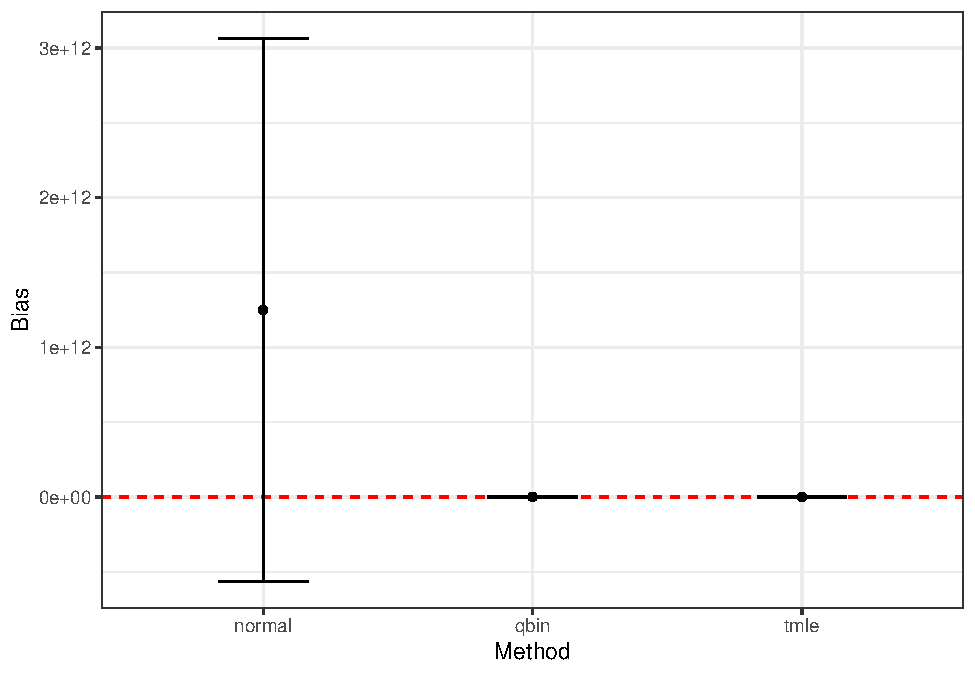
\includegraphics{simulation_files/figure-latex/sim-results-1.pdf}

\begin{Shaded}
\begin{Highlighting}[]
\FunctionTok{ggplot}\NormalTok{(}\FunctionTok{tidy}\NormalTok{(ss1, }\AttributeTok{stats =} \StringTok{"mse"}\NormalTok{), }\FunctionTok{aes}\NormalTok{(}\AttributeTok{x =}\NormalTok{ method, }\AttributeTok{y =}\NormalTok{ est, }\AttributeTok{ymin =}\NormalTok{ lower, }\AttributeTok{ymax =}\NormalTok{ upper)) }\SpecialCharTok{+}
  \FunctionTok{geom\_hline}\NormalTok{(}\AttributeTok{yintercept =} \DecValTok{0}\NormalTok{, }\AttributeTok{color =} \StringTok{"red"}\NormalTok{, }\AttributeTok{lty =} \StringTok{"dashed"}\NormalTok{) }\SpecialCharTok{+}
  \FunctionTok{geom\_point}\NormalTok{() }\SpecialCharTok{+}
  \FunctionTok{geom\_errorbar}\NormalTok{(}\AttributeTok{width =} \DecValTok{1} \SpecialCharTok{/} \DecValTok{3}\NormalTok{) }\SpecialCharTok{+}
  \FunctionTok{theme\_bw}\NormalTok{() }\SpecialCharTok{+}
  \FunctionTok{labs}\NormalTok{(}\AttributeTok{x =} \StringTok{"Method"}\NormalTok{, }\AttributeTok{y =} \StringTok{"MSE"}\NormalTok{)}
\end{Highlighting}
\end{Shaded}

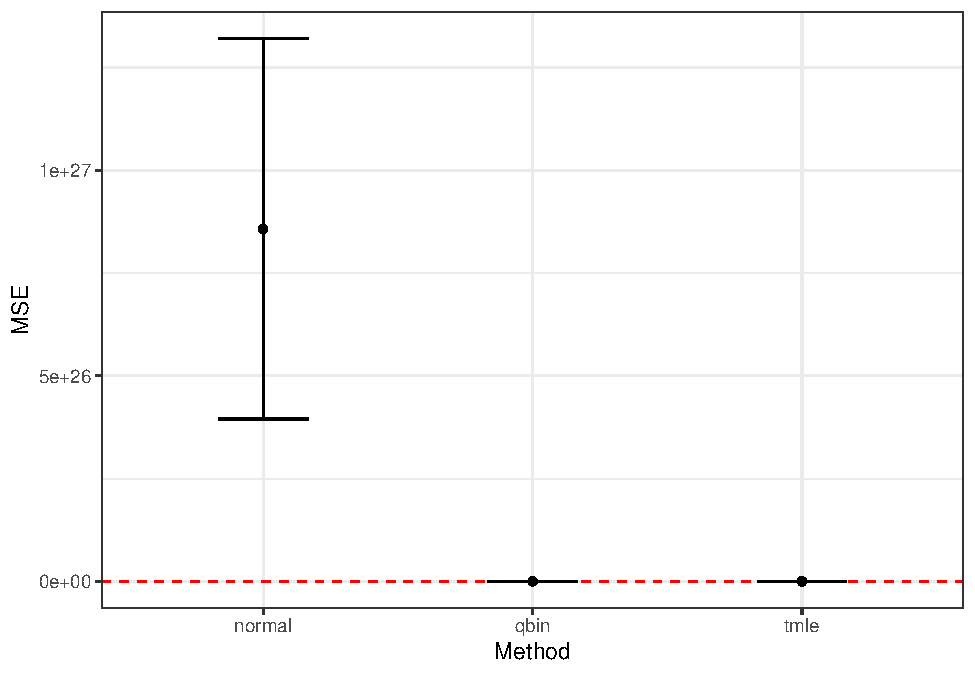
\includegraphics{simulation_files/figure-latex/sim-results-2.pdf}

\begin{Shaded}
\begin{Highlighting}[]
\FunctionTok{ggplot}\NormalTok{(}\FunctionTok{tidy}\NormalTok{(ss1, }\AttributeTok{stats =} \StringTok{"becover"}\NormalTok{), }\FunctionTok{aes}\NormalTok{(}\AttributeTok{x =}\NormalTok{ method, }\AttributeTok{y =}\NormalTok{ est, }\AttributeTok{ymin =}\NormalTok{ lower, }\AttributeTok{ymax =}\NormalTok{ upper)) }\SpecialCharTok{+}
  \FunctionTok{geom\_hline}\NormalTok{(}\AttributeTok{yintercept =} \FloatTok{0.95}\NormalTok{, }\AttributeTok{color =} \StringTok{"red"}\NormalTok{, }\AttributeTok{lty =} \StringTok{"dashed"}\NormalTok{) }\SpecialCharTok{+}
  \FunctionTok{geom\_point}\NormalTok{() }\SpecialCharTok{+}
  \FunctionTok{geom\_errorbar}\NormalTok{(}\AttributeTok{width =} \DecValTok{1} \SpecialCharTok{/} \DecValTok{3}\NormalTok{) }\SpecialCharTok{+}
  \FunctionTok{theme\_bw}\NormalTok{() }\SpecialCharTok{+}
  \FunctionTok{labs}\NormalTok{(}\AttributeTok{x =} \StringTok{"Method"}\NormalTok{, }\AttributeTok{y =} \StringTok{"Bias{-}eliminated Coverage"}\NormalTok{)}
\end{Highlighting}
\end{Shaded}

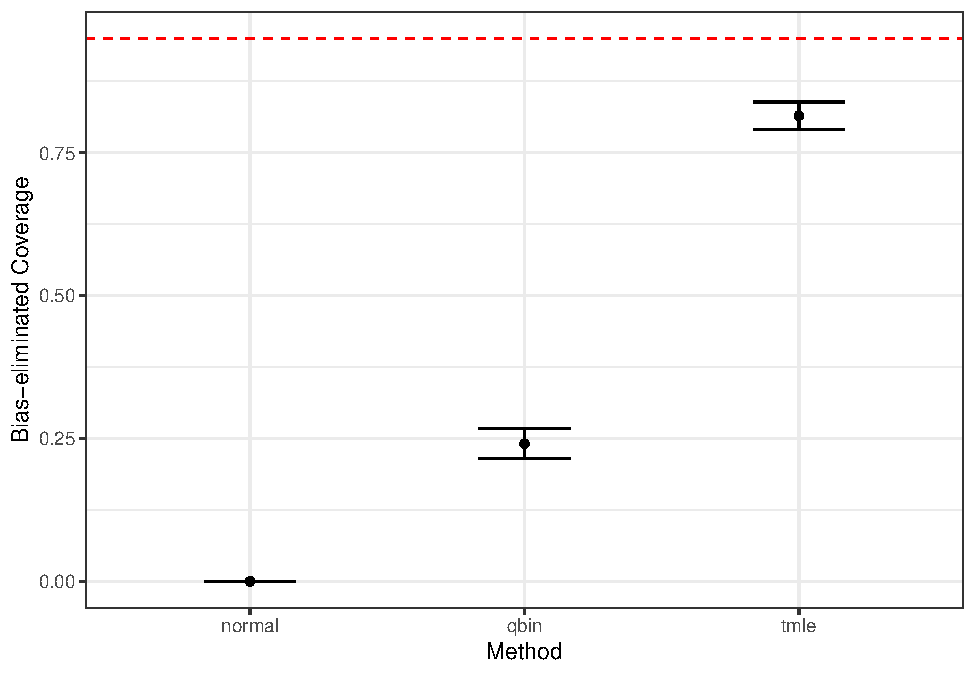
\includegraphics{simulation_files/figure-latex/sim-results-3.pdf}

\begin{Shaded}
\begin{Highlighting}[]
\FunctionTok{ggplot}\NormalTok{(}\FunctionTok{tidy}\NormalTok{(ss1, }\AttributeTok{stats =} \StringTok{"relerror"}\NormalTok{), }\FunctionTok{aes}\NormalTok{(}\AttributeTok{x =}\NormalTok{ method, }\AttributeTok{y =}\NormalTok{ est, }\AttributeTok{ymin =}\NormalTok{ lower, }\AttributeTok{ymax =}\NormalTok{ upper)) }\SpecialCharTok{+}
  \FunctionTok{geom\_hline}\NormalTok{(}\AttributeTok{yintercept =} \DecValTok{0}\NormalTok{, }\AttributeTok{color =} \StringTok{"red"}\NormalTok{, }\AttributeTok{lty =} \StringTok{"dashed"}\NormalTok{) }\SpecialCharTok{+}
  \FunctionTok{geom\_point}\NormalTok{() }\SpecialCharTok{+}
  \FunctionTok{geom\_errorbar}\NormalTok{(}\AttributeTok{width =} \DecValTok{1} \SpecialCharTok{/} \DecValTok{3}\NormalTok{) }\SpecialCharTok{+}
  \FunctionTok{theme\_bw}\NormalTok{() }\SpecialCharTok{+}
  \FunctionTok{labs}\NormalTok{(}\AttributeTok{x =} \StringTok{"Method"}\NormalTok{, }\AttributeTok{y =} \StringTok{"Relative Error"}\NormalTok{)}
\end{Highlighting}
\end{Shaded}

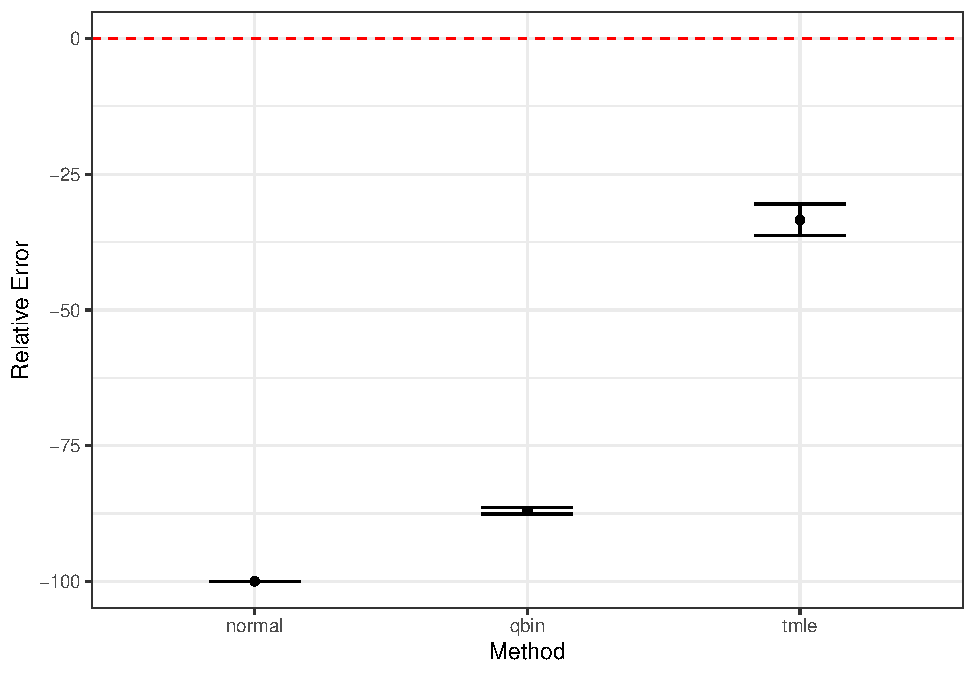
\includegraphics{simulation_files/figure-latex/sim-results-4.pdf}

\subsection{Save results}\label{save-results}

\begin{Shaded}
\begin{Highlighting}[]
\FunctionTok{library}\NormalTok{(ggplot2)}
\FunctionTok{library}\NormalTok{(patchwork)  }\CommentTok{\# for side{-}by{-}side layout}
\FunctionTok{library}\NormalTok{(rsimsum)}

\FunctionTok{library}\NormalTok{(forcats)}
\NormalTok{bias\_df }\OtherTok{\textless{}{-}} \FunctionTok{tidy}\NormalTok{(ss1, }\AttributeTok{stats =} \StringTok{"bias"}\NormalTok{) }\SpecialCharTok{\%\textgreater{}\%}
  \FunctionTok{mutate}\NormalTok{(}\AttributeTok{method =} \FunctionTok{fct\_recode}\NormalTok{(method,}
                             \StringTok{"IPW (Normal)"} \OtherTok{=} \StringTok{"normal"}\NormalTok{,}
                             \StringTok{"IPW (Quantile Binning)"} \OtherTok{=} \StringTok{"qbin"}\NormalTok{,}
                             \StringTok{"TMLE (Shift)"} \OtherTok{=} \StringTok{"tmle"}\NormalTok{))}

\CommentTok{\# Then use bias\_df in the plot}
\NormalTok{p1 }\OtherTok{\textless{}{-}} \FunctionTok{ggplot}\NormalTok{(bias\_df, }\FunctionTok{aes}\NormalTok{(}\AttributeTok{x =}\NormalTok{ method, }\AttributeTok{y =}\NormalTok{ est, }\AttributeTok{ymin =}\NormalTok{ lower, }\AttributeTok{ymax =}\NormalTok{ upper)) }\SpecialCharTok{+}
  \FunctionTok{geom\_point}\NormalTok{() }\SpecialCharTok{+}
  \FunctionTok{geom\_errorbar}\NormalTok{(}\AttributeTok{width =} \FloatTok{0.2}\NormalTok{) }\SpecialCharTok{+}
  \FunctionTok{geom\_hline}\NormalTok{(}\AttributeTok{yintercept =} \DecValTok{0}\NormalTok{, }\AttributeTok{linetype =} \StringTok{"dashed"}\NormalTok{) }\SpecialCharTok{+}
  \FunctionTok{labs}\NormalTok{(}\AttributeTok{y =} \StringTok{"Bias"}\NormalTok{, }\AttributeTok{x =} \StringTok{""}\NormalTok{) }\SpecialCharTok{+}
  \FunctionTok{theme\_bw}\NormalTok{(}\AttributeTok{base\_size =} \DecValTok{12}\NormalTok{) }\SpecialCharTok{+}
  \FunctionTok{theme}\NormalTok{(}\AttributeTok{panel.grid =} \FunctionTok{element\_blank}\NormalTok{(),}
        \AttributeTok{axis.text.x =} \FunctionTok{element\_text}\NormalTok{(}\AttributeTok{angle =} \DecValTok{20}\NormalTok{, }\AttributeTok{hjust =} \DecValTok{1}\NormalTok{))}

\NormalTok{mse\_df }\OtherTok{\textless{}{-}} \FunctionTok{tidy}\NormalTok{(ss1, }\AttributeTok{stats =} \StringTok{"mse"}\NormalTok{) }\SpecialCharTok{\%\textgreater{}\%}
  \FunctionTok{mutate}\NormalTok{(}\AttributeTok{method =} \FunctionTok{fct\_recode}\NormalTok{(method,}
                             \StringTok{"IPW (Normal)"} \OtherTok{=} \StringTok{"normal"}\NormalTok{,}
                             \StringTok{"IPW (Quantile Binning)"} \OtherTok{=} \StringTok{"qbin"}\NormalTok{,}
                             \StringTok{"TMLE (Shift)"} \OtherTok{=} \StringTok{"tmle"}\NormalTok{))}

\NormalTok{p2 }\OtherTok{\textless{}{-}} \FunctionTok{ggplot}\NormalTok{(mse\_df, }\FunctionTok{aes}\NormalTok{(}\AttributeTok{x =}\NormalTok{ method, }\AttributeTok{y =}\NormalTok{ est, }\AttributeTok{ymin =}\NormalTok{ lower, }\AttributeTok{ymax =}\NormalTok{ upper)) }\SpecialCharTok{+}
  \FunctionTok{geom\_point}\NormalTok{() }\SpecialCharTok{+}
  \FunctionTok{geom\_errorbar}\NormalTok{(}\AttributeTok{width =} \FloatTok{0.2}\NormalTok{) }\SpecialCharTok{+}
  \FunctionTok{geom\_hline}\NormalTok{(}\AttributeTok{yintercept =} \DecValTok{0}\NormalTok{, }\AttributeTok{linetype =} \StringTok{"dashed"}\NormalTok{) }\SpecialCharTok{+}
  \FunctionTok{labs}\NormalTok{(}\AttributeTok{y =} \StringTok{"Mean squared error"}\NormalTok{, }\AttributeTok{x =} \StringTok{""}\NormalTok{) }\SpecialCharTok{+}
  \FunctionTok{theme\_bw}\NormalTok{(}\AttributeTok{base\_size =} \DecValTok{12}\NormalTok{) }\SpecialCharTok{+}
  \FunctionTok{theme}\NormalTok{(}\AttributeTok{panel.grid =} \FunctionTok{element\_blank}\NormalTok{(),}
        \AttributeTok{axis.text.x =} \FunctionTok{element\_text}\NormalTok{(}\AttributeTok{angle =} \DecValTok{20}\NormalTok{, }\AttributeTok{hjust =} \DecValTok{1}\NormalTok{))}

\NormalTok{becover\_df }\OtherTok{\textless{}{-}} \FunctionTok{tidy}\NormalTok{(ss1, }\AttributeTok{stats =} \StringTok{"becover"}\NormalTok{) }\SpecialCharTok{\%\textgreater{}\%}
  \FunctionTok{mutate}\NormalTok{(}\AttributeTok{method =} \FunctionTok{fct\_recode}\NormalTok{(method,}
                             \StringTok{"IPW (Normal)"} \OtherTok{=} \StringTok{"normal"}\NormalTok{,}
                             \StringTok{"IPW (Quantile Binning)"} \OtherTok{=} \StringTok{"qbin"}\NormalTok{,}
                             \StringTok{"TMLE (Shift)"} \OtherTok{=} \StringTok{"tmle"}\NormalTok{))}

\NormalTok{p3 }\OtherTok{\textless{}{-}} \FunctionTok{ggplot}\NormalTok{(becover\_df, }\FunctionTok{aes}\NormalTok{(}\AttributeTok{x =}\NormalTok{ method, }\AttributeTok{y =}\NormalTok{ est, }\AttributeTok{ymin =}\NormalTok{ lower, }\AttributeTok{ymax =}\NormalTok{ upper)) }\SpecialCharTok{+}
  \FunctionTok{geom\_point}\NormalTok{() }\SpecialCharTok{+}
  \FunctionTok{geom\_errorbar}\NormalTok{(}\AttributeTok{width =} \FloatTok{0.2}\NormalTok{) }\SpecialCharTok{+}
  \FunctionTok{geom\_hline}\NormalTok{(}\AttributeTok{yintercept =} \FloatTok{0.95}\NormalTok{, }\AttributeTok{linetype =} \StringTok{"dashed"}\NormalTok{) }\SpecialCharTok{+}
  \FunctionTok{labs}\NormalTok{(}\AttributeTok{y =} \StringTok{"Bias{-}eliminated Coverage (95\%)"}\NormalTok{, }\AttributeTok{x =} \StringTok{""}\NormalTok{) }\SpecialCharTok{+}
  \FunctionTok{theme\_bw}\NormalTok{(}\AttributeTok{base\_size =} \DecValTok{12}\NormalTok{) }\SpecialCharTok{+}
  \FunctionTok{theme}\NormalTok{(}\AttributeTok{panel.grid =} \FunctionTok{element\_blank}\NormalTok{(),}
        \AttributeTok{axis.text.x =} \FunctionTok{element\_text}\NormalTok{(}\AttributeTok{angle =} \DecValTok{20}\NormalTok{, }\AttributeTok{hjust =} \DecValTok{1}\NormalTok{))}

\CommentTok{\# Combine plots side by side}
\NormalTok{combined\_plot }\OtherTok{\textless{}{-}}\NormalTok{ p1 }\SpecialCharTok{+}\NormalTok{ p2 }\SpecialCharTok{+}\NormalTok{ p3 }\SpecialCharTok{+} \FunctionTok{plot\_layout}\NormalTok{(}\AttributeTok{ncol =} \DecValTok{3}\NormalTok{)}

\CommentTok{\# Save to PNG}
\FunctionTok{ggsave}\NormalTok{(}\StringTok{"sim\_summary\_bw.png"}\NormalTok{, combined\_plot, }\AttributeTok{width =} \DecValTok{10}\NormalTok{, }\AttributeTok{height =} \DecValTok{4}\NormalTok{, }\AttributeTok{dpi =} \DecValTok{600}\NormalTok{)}
\end{Highlighting}
\end{Shaded}

\subsubsection{Trace plot}\label{trace-plot}

This plot shows the cumulative mean of estimates over simulations,
indicating convergence.

\begin{Shaded}
\begin{Highlighting}[]
\CommentTok{\# Plotting the estimates}
\NormalTok{true\_logOR }\OtherTok{\textless{}{-}} \FloatTok{0.4}  \CommentTok{\# True conditional log{-}odds ratio}

\CommentTok{\# Cumulative mean}
\NormalTok{results}\SpecialCharTok{$}\NormalTok{cum\_mean\_normal }\OtherTok{\textless{}{-}} \FunctionTok{cumsum}\NormalTok{(results}\SpecialCharTok{$}\NormalTok{normal) }\SpecialCharTok{/} \FunctionTok{seq\_len}\NormalTok{(}\FunctionTok{nrow}\NormalTok{(results))}
\NormalTok{results}\SpecialCharTok{$}\NormalTok{cum\_mean\_qbin }\OtherTok{\textless{}{-}} \FunctionTok{cumsum}\NormalTok{(results}\SpecialCharTok{$}\NormalTok{qbin) }\SpecialCharTok{/} \FunctionTok{seq\_len}\NormalTok{(}\FunctionTok{nrow}\NormalTok{(results))}
\NormalTok{results\_tmle}\SpecialCharTok{$}\NormalTok{cum\_mean\_tmle }\OtherTok{\textless{}{-}} \FunctionTok{cumsum}\NormalTok{(results\_tmle}\SpecialCharTok{$}\NormalTok{logOR\_tmle) }\SpecialCharTok{/} \FunctionTok{seq\_len}\NormalTok{(}\FunctionTok{nrow}\NormalTok{(results\_tmle))}

\CommentTok{\# Add iteration index}
\NormalTok{results}\SpecialCharTok{$}\NormalTok{iteration }\OtherTok{\textless{}{-}} \FunctionTok{seq\_len}\NormalTok{(}\FunctionTok{nrow}\NormalTok{(results))}
\NormalTok{results\_tmle}\SpecialCharTok{$}\NormalTok{iteration }\OtherTok{\textless{}{-}} \FunctionTok{seq\_len}\NormalTok{(}\FunctionTok{nrow}\NormalTok{(results\_tmle))}

\CommentTok{\# Combine for plotting}
\NormalTok{cum\_long }\OtherTok{\textless{}{-}} \FunctionTok{rbind}\NormalTok{(}
  \FunctionTok{data.frame}\NormalTok{(}\AttributeTok{iteration =}\NormalTok{ results}\SpecialCharTok{$}\NormalTok{iteration, }\AttributeTok{cum\_mean =}\NormalTok{ results}\SpecialCharTok{$}\NormalTok{cum\_mean\_normal, }\AttributeTok{method =} \StringTok{"Normal Model"}\NormalTok{),}
  \FunctionTok{data.frame}\NormalTok{(}\AttributeTok{iteration =}\NormalTok{ results}\SpecialCharTok{$}\NormalTok{iteration, }\AttributeTok{cum\_mean =}\NormalTok{ results}\SpecialCharTok{$}\NormalTok{cum\_mean\_qbin, }\AttributeTok{method =} \StringTok{"Quantile Binning"}\NormalTok{),}
  \FunctionTok{data.frame}\NormalTok{(}\AttributeTok{iteration =}\NormalTok{ results\_tmle}\SpecialCharTok{$}\NormalTok{iteration, }\AttributeTok{cum\_mean =}\NormalTok{ results\_tmle}\SpecialCharTok{$}\NormalTok{cum\_mean\_tmle, }\AttributeTok{method =} \StringTok{"TMLE"}\NormalTok{)}
\NormalTok{)}

\CommentTok{\# Plot}
\FunctionTok{library}\NormalTok{(ggplot2)}
\FunctionTok{ggplot}\NormalTok{(cum\_long, }\FunctionTok{aes}\NormalTok{(}\AttributeTok{x =}\NormalTok{ iteration, }\AttributeTok{y =}\NormalTok{ cum\_mean, }\AttributeTok{color =}\NormalTok{ method)) }\SpecialCharTok{+}
  \FunctionTok{geom\_line}\NormalTok{(}\AttributeTok{size =} \DecValTok{1}\NormalTok{) }\SpecialCharTok{+}
  \FunctionTok{geom\_hline}\NormalTok{(}\AttributeTok{yintercept =}\NormalTok{ true\_logOR, }\AttributeTok{linetype =} \StringTok{"dashed"}\NormalTok{, }\AttributeTok{color =} \StringTok{"black"}\NormalTok{) }\SpecialCharTok{+}
  \FunctionTok{labs}\NormalTok{(}
    \AttributeTok{title =} \StringTok{"Cumulative Mean of log(OR) Over Simulations"}\NormalTok{,}
    \AttributeTok{x =} \StringTok{"Simulation Iteration"}\NormalTok{,}
    \AttributeTok{y =} \StringTok{"Cumulative Mean of log(OR)"}\NormalTok{,}
    \AttributeTok{color =} \StringTok{"Estimator"}
\NormalTok{  ) }\SpecialCharTok{+}
  \FunctionTok{theme\_minimal}\NormalTok{()}
\end{Highlighting}
\end{Shaded}

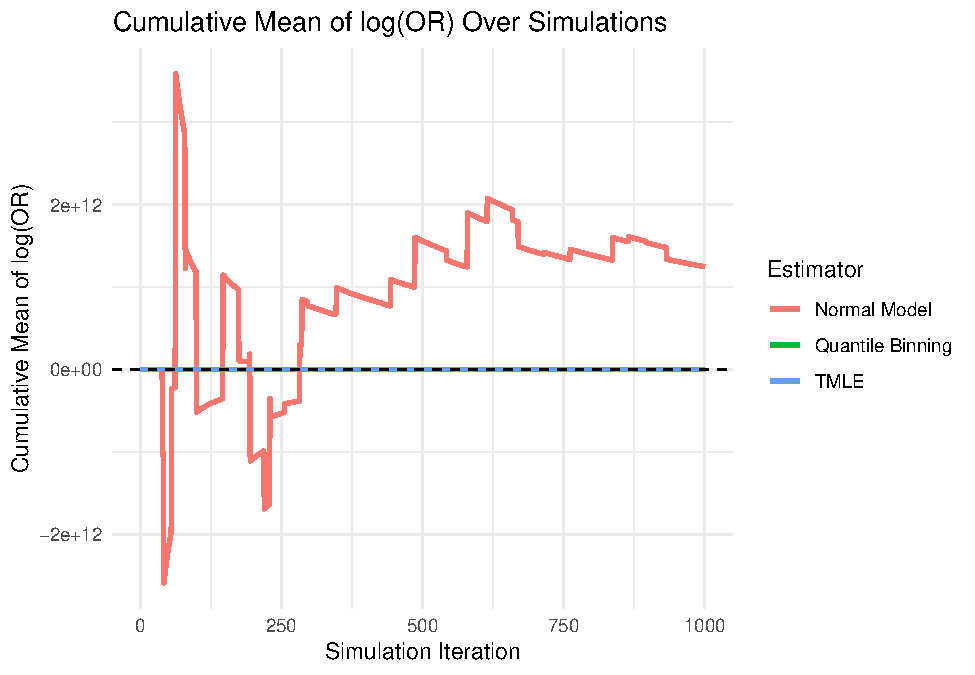
\includegraphics{simulation_files/figure-latex/sim-plot-1.pdf}

\end{document}
